\documentclass[a4paper,12pt]{article}
\usepackage{graphicx}
\usepackage{graphics}
\usepackage{amsbsy}
\usepackage{cmmib57}
\usepackage{amssymb}
%\usepackage{algorithm2e}
\usepackage[ruled,vlined]{algorithm2e}
%\usepackage{hyperref}

\usepackage{dsfont} % real
\usepackage{amsmath}
\usepackage{upref}
\usepackage{multicol}
\usepackage{caption}

%%\usepackage[isolatin,cp1251]{inputenc}
%%\usepackage[english,russian]{babel}

\usepackage[utf8]{inputenc}
\usepackage[russian]{babel}
\usepackage[T1]{fontenc}
\usepackage{verbatim}

\graphicspath{{img/}}

%% Page Style
%\headheight=14pt \headsep=14pt \textheight=255mm \topskip=0pt
%\textwidth=165mm \oddsidemargin=5mm
%\evensidemargin=-5mm%0mm
%\parindent1.1cm
%\topmargin=-15mm \footskip=0pt
%\parindent1.1cm
%\pagestyle{empty}

\usepackage[left=2.5cm,right=2cm,top=2.5cm, bottom=2.5cm]{geometry}%поля

\usepackage{makeidx}
%\usepackage[a5paper,%
%twosideshift=12pt,%
%body={114 true mm,170 true mm},%
%totalheight=178true mm%
%]{geometry}

\DeclareGraphicsRule{.bmp}{bmp}{}{}

%%%% sectioning and headings
\numberwithin{equation}{section}

\newif\iffirstinpart
\firstinpartfalse

\usepackage[bf,small,center,compact,aftersep,indentfirst,clearempty,pagestyles]{titlesec}
%%%
\titlelabel{\thetitle.\quad}

\newcommand{\partbreak}{\cleardoublepage\thispagestyle{empty}\global\firstinparttrue\relax}
\newcommand{\chapterbreak}{\iffirstinpart \relax\else\clearpage \fi\relax%%
  \thispagestyle{empty}\global\firstinpartfalse\typeout{chapterbreak}}

% Table of contents
\makeatletter
\renewcommand{\tableofcontents}{\chaptera{Содержание}\@starttoc{toc}}
\renewcommand{\@dotsep}{2}
\renewcommand{\l@section}{\@dottedtocline{1}{1.5em}{2.3em}}
\newcommand{\l@chapter}{\vspace{0.5cm}\@dottedtocline{0}{0em}{2.3em}}
\newcommand{\l@chaptera}{\vspace{0.5cm}\@dottedtocline{0}{0em}{2.3em}}
\makeatother

%% Environments
\newcounter{chapter}
\newcounter{chaptera}

\renewcommand{\thechapter}{\arabic{chapter}}
\renewcommand{\thechaptera}{\arabic{chaptera}}
\renewcommand{\thesection}{\arabic{section}}
\renewcommand{\thesubsection}{\thesection.\arabic{subsection}}

\numberwithin{equation}{section}
\numberwithin{table}{chapter}
\numberwithin{section}{chapter}

\newcommand{\chaptera}[1]{%
\clearpage\refstepcounter{chaptera}
\addcontentsline{toc}{chaptera}{#1}
{\huge\bfseries #1 \Large \vskip14pt}}

\newcommand{\chapter}[1]{%
\clearpage\refstepcounter{chapter}
\setcounter{section}{0}
\addcontentsline{toc}{chapter}{\textbf{\thechapter.} #1}
{\huge\bfseries  \thechapter\ \ #1 \Large \vskip 1cm}}

\renewcommand{\section}[1]{%
\refstepcounter{section}%
\setcounter{subsection}{0}
\addcontentsline{toc}{section}{\thesection. #1} {\vskip 14pt
\LARGE\bfseries\,\thesection\; #1\Large\vskip 10pt}}

\renewcommand{\subsection}[1]
{\refstepcounter{subsection}%
{\vskip 10pt \bfseries\,\thesubsection\;  #1}}

%%%%

\setcounter{tocdepth}{1}
\emergencystretch=1.25pt\relax
\hfuzz=0.5pt\relax
\tolerance=250\relax

\newcommand{\ac}[1]{#1}
\newcommand{\acs}[1]{#1}
%%%-----------------------------------------------------------------/

\newenvironment{proof}[1]{\samepage$\nabla$ \textit{Доказательство.} #1}{\\ \rightline{$\Delta$}}

\makeindex

\setlength{\abovedisplayskip}{2.5pt}
\setlength{\belowdisplayskip}{2.5pt}
\setlength{\abovedisplayshortskip}{1.25pt}
\setlength{\belowdisplayshortskip}{1.25pt} \setlength{\jot}{0.0pt}
%\theoremstyle{plain} \setlength{\theorempreskipamount}{1mm}
%\setlength{\theorempostskipamount}{1mm}

% Define Theorem
\newcounter{theorem}[section]\numberwithin{theorem}{section}
\newenvironment{theorem}[1][0]{\par\vspace{3mm plus 1mm minus 1mm}\noindent%
\refstepcounter{theorem}%
\ifx0#1{\bfseries Теорема \thesection.\arabic{theorem}. \hskip 8pt}%
\else{\bfseries Теорема \thesection.\arabic{theorem} {\normalfont(#1)}.}%
\fi\itshape } {\normalfont\par\vspace{2mm}}

% Define Example
\newcounter{example}[section]\numberwithin{example}{section}
\newenvironment{example}[1][0]{\par\vspace{3mm plus 1mm minus 1mm}\noindent%
\refstepcounter{example}%
\ifx0#1{\bfseries Пример \thesection.\arabic{example}. \hskip 8pt}%
\else{\bfseries Пример \thesection.\arabic{example} {\normalfont(#1)}.}%
\fi\itshape } {\normalfont\par\vspace{2mm}}

% Define Lemma
\newcounter{lemma}[section]\numberwithin{lemma}{section}
\newenvironment{lemma}[1][0]{\par\vspace{3mm plus 1mm minus 1mm}\noindent%
\refstepcounter{lemma}%
\ifx0#1{\bfseries Лемма \thesection.\arabic{lemma}.\hskip 8pt}%
\else{\bfseries Лемма \thesection.\arabic{lemma} {\normalfont(#1)}.}%
\fi\itshape } {\normalfont\par\vspace{2mm}}

% Define Definition
\newcounter{definition}[section]\numberwithin{definition}{section}
\newenvironment{definition}[1][0]{\par\vspace{3mm plus 1mm minus 1mm}\noindent%
\refstepcounter{definition}%
\ifx0#1{\bfseries Определение \thesection.\arabic{definition}.\hskip 8pt}%
\else{\bfseries Определение \thesection.\arabic{definition} {\normalfont(#1)}.}%
\fi\itshape } {\normalfont\par\vspace{2mm}}

% Define Zamechanie
\newcounter{zam}[section]\numberwithin{zam}{section}
\newenvironment{zam}[1][0]{\par\vspace{3mm plus 1mm minus 1mm}\noindent%
\refstepcounter{zam}%
\ifx0#1{\bfseries Замечание \thesection.\arabic{zam}.\hskip 8pt}%
\else{\bfseries Замечание \thesection.\arabic{zam} {\normalfont(#1)}.}%
\fi\itshape } {\normalfont\par\vspace{2mm}}

% Define Primer
\newcounter{prim}[section]\numberwithin{prim}{section}
\newenvironment{prim}[1][0]{\par\vspace{3mm plus 1mm minus 1mm}\noindent%
\refstepcounter{prim}%
\ifx0#1{\bfseries Пример \thesection.\arabic{prim}. }%
\else{\bfseries Пример \thesection.\arabic{prim} {\normalfont(#1)}.}%
\fi\itshape } {\normalfont\par\vspace{2mm}}

% Define Algorithm
\newcounter{alg}[section]\numberwithin{alg}{section}
\newenvironment{alg}[1][0]{\par\vspace{3mm plus 1mm minus 1mm}\noindent%
\refstepcounter{alg}%
\ifx0#1{\bfseries Алгоритм \thesection.\arabic{alg}. \hskip 8pt}%
\else{\bfseries Алгоритм \thesection.\arabic{alg} {\normalfont(#1)}.}%
\fi\itshape } {\normalfont\par\vspace{2mm}}

% Define PrimerDopoln
\newcounter{prm}[section]\numberwithin{prm}{section}
\newenvironment{prm}[1][0]{\par\vspace{3mm plus 1mm minus 1mm}\noindent%
\refstepcounter{prm}%
\ifx0#1{\bfseries Пример \arabic{prm}. }%
\else{\bfseries Пример \arabic{prm} {\normalfont(#1)}.}%
\fi\itshape } {\normalfont\par\vspace{2mm}}

% Define DefinitionDopoln
\newcounter{defn}[section]\numberwithin{defn}{section}
\newenvironment{defn}[1][0]{\par\vspace{3mm plus 1mm minus 1mm}\noindent%
\refstepcounter{defn}%
\ifx0#1{\bfseries Определение \arabic{defn}.\hskip 8pt}%
\else{\bfseries Определение \arabic{defn} {\normalfont(#1)}.}%
\fi\itshape } {\normalfont\par\vspace{2mm}}

% Define TheoremDopoln
\newcounter{thm}[section]%\numberwithin{theorem}{section}
\newenvironment{thm}[1][0]{\par\vspace{3mm plus 1mm minus 1mm}\noindent%
\refstepcounter{thm}%
\ifx0#1{\bfseries Теорема \arabic{thm}. \hskip 8pt}%
\else{\bfseries Теорема \arabic{thm} {\normalfont(#1)}.}%
\fi\itshape } {\normalfont\par\vspace{2mm}}

%\newcommand{\contsection}[1]{\begin{center}#1\end{center}}
%\newcommand{\contline}[2]{\noindent#2\dotfill\pageref{#1}\vspace{1mm}\\}
%\newcommand{\contlines}[2]{\noindent#2\dotfill#1\vspace{1mm}\\}

\newcounter{conditioncounter}
\newenvironment{conditionsnum}{\begin{list}
{\rm(\arabic{conditioncounter})} {\usecounter{conditioncounter}
\leftmargin=10mm \labelsep=3mm \labelwidth=15mm \topsep=0pt plus
1pt
\parsep=0pt plus 1pt}}
{\end{list}}

\newenvironment{conditionslet}{\begin{list}
{\rm(\alph{conditioncounter})} {\usecounter{conditioncounter}
\leftmargin=10mm \labelsep=3mm \labelwidth=15mm \topsep=0pt plus
1pt
\parsep=0pt plus 1pt}}
{\end{list}}

\newcommand{\impl}[2]{{\rm(#1)} $\Rightarrow$ {\rm(#2)}}

\newcounter{bibl}
\setcounter{bibl}{0}
\newcommand{\bibl}[1]
  {\item[\refstepcounter{bibl}{[\thebibl]}\label{bibl:#1}]}
\renewcommand{\cite}[1]{[\ref{bibl:#1}]}
\newcommand{\cites}[1]{\ref{bibl:#1}}
%\newcommand{\nl}{\mbox{}\\}

\renewcommand{\arraystretch}{1.3}
\setlength{\arraycolsep}{1pt}


%%%%рисунки
%\newcounter{ё}[chapter]
\numberwithin{figure}{chapter}
\renewenvironment{figure}[2]{\vskip14pt%
\refstepcounter{figure}%
\center #2 \\
\large \center Рис. \thefigure:\: #1 \Large}
{\vskip14pt}%%%%%%%%%%%%%%%%%%%%

\renewcommand{\phi}{\varphi}
\newcommand{\dd}{\partial}

% Переопределение le ge в русских традициях
\renewcommand{\le}{\leqslant}
%\renewcommand{\leq}{\leqslant}
\renewcommand{\ge}{\geqslant}
%\renewcommand{\geq}{\geqslant}

\begin{document}
	\Large
	\sloppy \baselineskip=8mm 	
	\tableofcontents
\newpage
% В этом файле следует писать текст работы, разбивая его на
% разделы (section), подразделы (subsection) и, если нужно,
% главы (chapter).

% Предварительно следует указать необходимую информацию
% в файле SETUP.tex

%% В этот файл не предполагается вносить изменения

\input{SETUP.tex}

\usepackage {amsmath}      % Больше математики
\usepackage {amssymb}
\usepackage {textcase}     % Преобразование к верхнему регистру
\usepackage {indentfirst}  % Красная строка первого абзаца в разделе
\usepackage {fancyvrb}     % Листинги: определяем своё окружение Verb

\DefineVerbatimEnvironment% с уменьшенным шрифтом
	{Verb}{Verbatim}
	{fontsize=\small}

% Вставка рисунков
\usepackage {graphicx}

% Общее оформление
\input{core/appearance.tex}

% Стили для окружений типа Определение, Теорема...
\input{core/theorem_styles.tex}

% Титульный лист
\input{core/title_macro.tex}

% Команды для использования в тексте работы
\input{my_macro.tex}

\endinput

% Конец файла

\begin{document}
	
	\Intro
	
	Целью данной работы является описание выбора задачи для будущей магистерской диссертации и ее
	первоначальное изучение. 
	
	Направлением исследования для магистерской диссертации было выбрано развитие темы графов с нестандартной достижимостью, описанной в~\autocite{Mono}. Соответственно, в начале была рассмотрена сама теория и несколько частных задач с условиями на нестандартную достижимость в графах, далее они были проанализированы подробнее. Часть из них была сведена к задачам, уже описанным в~\autocite{Mono}, но также был выделен новый тип условий, не имеющий аналога среди рассмотренных прежде задач.
	
	Упомянутый тип условий был описан как глобальные условия на графах с нестандартной достижимостью, также были выделены отличия, не позволяющие свести глобальные условия к каким-либо уже рассмотренным в~\autocite{Mono}. 
	
	В качестве примера задачи с глобальным условием на достижимость подробно рассматривается задача с проверкой кратности количества дуг данного множества в пройденном пути. Для нее записывается формальная постановка задачи, приводится алгоритм построения вспомогательного графа и доказывается теорема о связи путей на исходном и вспомогательным графах. Т.о., показывается, что глобальные условия на достижимость являются частным случаем графов с нестандартной достижимостью. 
	
	Далее введём ряд стандартных определений теории графов, которыми будем пользоваться в данной работе. 
	
	\begin{mydefinition}
		Ориентированным графом, или орграфом, будем называть тройку $G(X,U,f)$, в которой:
		\begin{itemize}
			\item $X$ --- непустое множество вершин графа.
			\item $U$ --- множество дуг графа, возможно, пустое.
			\item $f:U\to X \times X$ --- отображение инцидентности, причём $f(u) = (x, y)$, где $u \in U$, $x, y \in X$, $x$ --- начальная вершина дуги $u$, а $y$ --- конечная.
		\end{itemize}
	\end{mydefinition}
	
	\begin{mydefinition}
		Рассмотрим пару отображений $p_1:X \times X\to X$, $p_2:X \times X\to X$:
		\begin{itemize}
			\item $p_1(x, y) = x$, $x = (p_1 \circ f)(u)$ --- начальная вершина дуги $u$,
			\item $p_2(x, y) = y$, $y = (p_2 \circ f)(u)$ --- концевая вершина дуги $u$.
		\end{itemize}
	\end{mydefinition}
	
	\begin{mydefinition}
		Отображение $\mu:\{1, 2, ... , n\} \to U$ такое, что 
		$(p_2 \circ f \circ \mu)(i) = (p_1 \circ f \circ \mu)(i + 1)$ при $i \in \{1, 2, ... , n-1\}$
		будем называть путём на графе $G$ длины $n$.
	\end{mydefinition}

	\begin{mydefinition}
		Перемещение по графу $G(X,U,f)$ в дискретном времени $t$ задаётся с помощью стохастической матрицы $P$, где $p_{ij}$ --- вероятность перехода из вершины $x_i$ в $x_j$.
		Такую матрицу будем называть матрицей вероятностей переходов или просто матрицей переходов.
	\end{mydefinition}
	
	\chapter{Теоретические основы глобальных условий на достижимость на графах}
		
	\section{Основные положения теории графов с нестандартной достижимостью}
	
	\begin{mydefinition}
		Графом с нестандартной достижимостью будем называть орграф $G(X,U,f)$, для которого верно:
		\begin{enumerate}
			\item Дуги разделены на множества $U_* = \{U_0, U_1, ... , U_m\}$ и $U^* = \{U^0, U^1, ... , U^k\}$, причём различные подмножества не пересекаются, a числа $k, m \in Z_+$ заранее известны.
			\item Определено отображение $\psi_\mu:N\to \overline{ [0; k] }$, называемое числовой характеристикой произвольного пути $\mu$.
			\item Задано формальное ограничение на достижимость пути.
		\end{enumerate}
	\end{mydefinition}
	
	Характеристика $\psi_\mu$ определяется рекуррентно по последней дуге пути $\mu$ с помощью некоторой заданной функции, a $\psi_\mu(0) = 0$.
	
	Можно выделить два типа формальных ограничений:
	\begin{itemize}
		\item Строгие: $\forall m (\psi_\mu(m) = j) \Longrightarrow (\mu(m+1) \in U^j) $, т.е. следующая дуга пути обязана принадлежать $U^j$.
		\item Нестрогие: $\forall m (\psi_\mu(m) = j) \& ([(p_2 \circ f \circ \mu)(m)]^+ \cap U^j \neq \emptyset) \Longrightarrow (\mu(m+1) \in U^j) $, т.е. следующая дуга пути обязана принадлежать $U^j$, только если есть хотя бы одна такая дуга.
	\end{itemize}
	
	Для графов с нестандартной достижимостью в~\autocite{Mono} предлагается строить вспомогательные графы, причём правила построения таких графов зависят от типа налагаемых условий на достижимость. 
	Также доказывается теорема о соответствии любого пути на вспомогательном графе допустимому пути на исходном графе. Благодаря этой теореме задача о поиске кратчайшего допустимого пути на исходном графе сводится к классической задаче поиска кратчайшего пути на вспомогательном графе.
	
	\begin{mydefinition}
		Пусть имеем некоторый путь $\mu$ из последовательных дуг $\{u_1, u_2, ... , u_{m-1}, u_m\}$. Любой путь, полученный отбрасыванием любого количества последних дуг пути подряд вида $\{u_1, u_2, ... , u_{m-n} \}$ будем называть префиксом пути $\mu$.
	\end{mydefinition}
	
	\begin{mydefinition}
		Будем говорить, что допустимый путь из последовательных дуг $\{u_1, u_2, ... , u_{m-1}, u_m\}$ является модульным, если любой его префикс также является допустимым. Соответственно, это свойство будем именовать модульностью допустимого пути. 
	\end{mydefinition}
	
	\section{Некоторые частные задачи на графах с нестандартной достижимостью}
	
	В данном разделе приводятся рассмотренные задачи на графах, достижимость путей в которых описывается теорией о графах с нестандартной достижимостью, либо будет описана в терминах данной теории в будущей магистерской работе. 
	
	\subsection{Задача о проходе по дугам невозрастающей длины}
	
	Рассмотрим ориентированный граф $G(X,U,f)$. Каждой дуге $u_i$ сопоставлено некоторое целое положительное число $l_i$, именуемое длиной данной дуги. Будем называть путь на введённом графе допустимым, если длины последовательных дуг данного пути образуют монотонную невозрастающую последовательность. Тогда задача о поиске кратчайшего пути(в смысле длины пути) на графе подразумевает поиск кратчайшего допустимого пути, все прочие пути не рассматриваются. 
	
	\begin{figure}
		\centering
		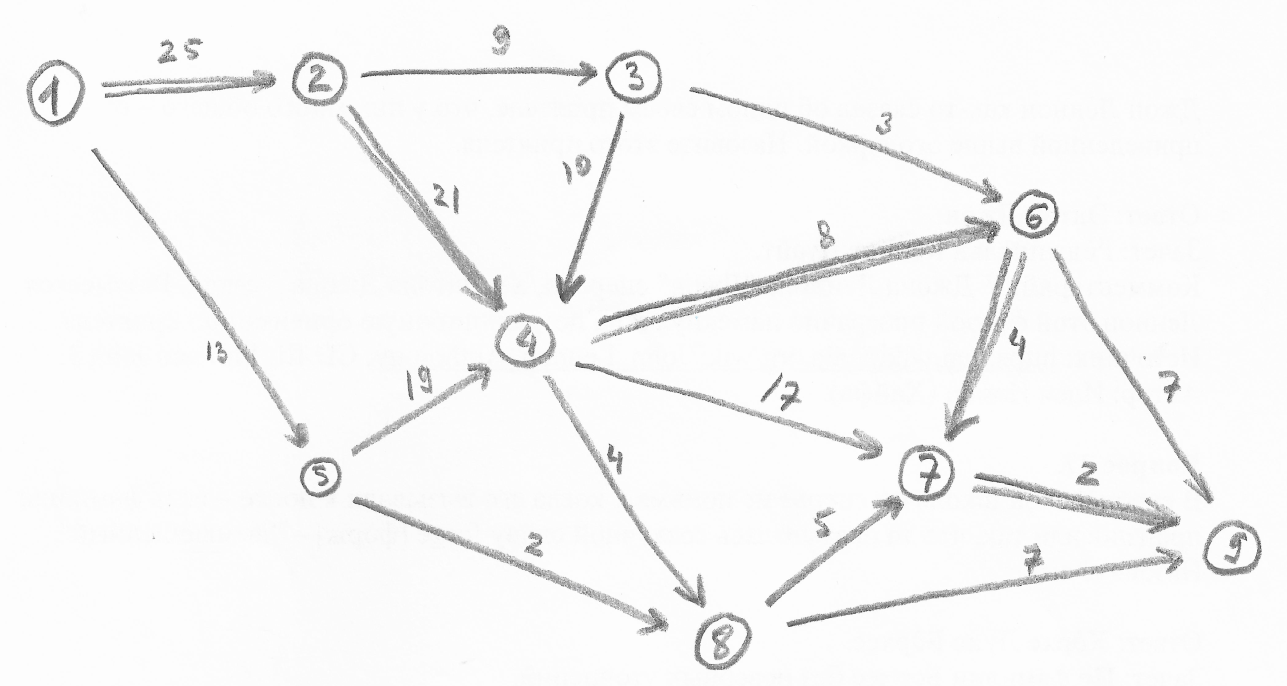
\includegraphics[width=0.9\textwidth]{img/1.png}
		\caption{Пример графа с условием о проходе по дугам невозрастающей длины; двойными стрелками обозначен допустимый кратчайший путь.}
		\label{fig:pic_1}
	\end{figure}
	
	Однако, условие этой задачи можно свести к описанному в~\autocite{Mono} условию вентильной достижимости с возрастанием-убыванием доступа на пути. Опишем соответствие подробней. В формулировке условия вентильной достижимости с возрастанием-убыванием доступа на пути $U_*$ пусто, дуги из $U$ разбиваются на $k$ непересекающихся подмножеств множества $U^*$; это можно провести, разделив всё множество $U$ на подмножества в соответствии с длинами $l_i$, ассоциированными с каждой дугой $u_i$. При этом $k = |\{ l_i : u_i \in U\}|$. Также нужно установить соответствие между индексами множеств $\in [1; k]$ и длинами дуг из них, сохранив при этом упорядоченность длин по возрастанию. Введём некоторое оторбажение $g:[1; k]\to \{ l_i : u_i \in U\}$, осуществляющее это соответствие. 
	
	Числовой характеристикой произвольного пути (в условиях задачи называемой порядком доступа на пути)
	$\psi_\mu$ тогда будет являться длина последней дуги пути. Соответственно, если $\psi_\mu(i) = j$, следующей дугой может быть только дуга $\in U_0 \cup ... \cup U_j$, т.е. некоторая дуга, длина которой не превышает $g(j)$. Т.о., требование монотонного невозрастания последовательности длин дуг записано через принадлежность дуг подмножествам. 
	
	После того, как установлено соответствие с условием вентильной достижимости с возрастанием-убыванием доступа на пути, можно использовать алгоритм построения вспомогательного графа для этой задачи и искать кратчайший допустимый путь с помощью, например, алгоритма Дейкстры на вспомогательном графе. 
	
	\subsection{Задача о допустимости пути только с числом дуг данного множества, кратным некоторому фиксированному числу}
	
	Вновь рассмотрим ориентированный граф $G(X,U,f)$. Теперь граф не имеет ассоциированных с дугами характеристик, и есть два непересекающихся множества дуг --- стандартные $U_s$ и остаточные $U_o$. Будем называть путь на графе $G$ допустимым, если в нем содержится количество остаточных дуг, кратное фиксированному целому числу $p$ ($|p| > 1$). Как и прежде, будем искать кратчайший(в смысле количества дуг) допустимый путь.
	
	\begin{figure}
		\centering
		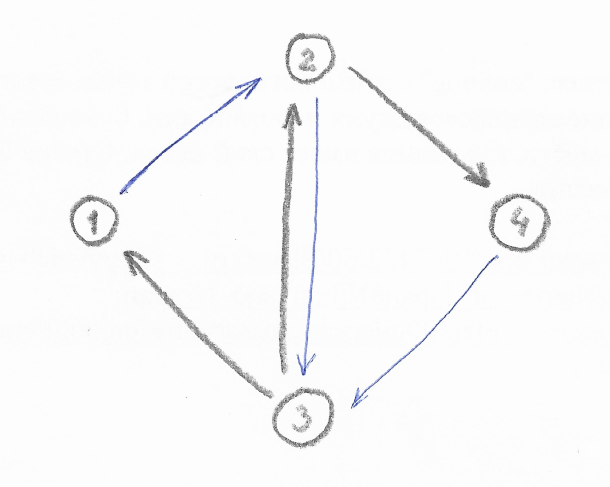
\includegraphics[width=0.6\textwidth]{img/2.png}
		\caption{Пример графа с допустимым путем только с числом дуг из $U_o$, кратным $p$; черные стрелки означают дуги из $U_s$, синие --- из $U_o$.}
		\label{fig:pic_2}
	\end{figure}
	
	К примеру, для рис.2 ясно, что кратчайший допустимый путь из 1-ой вершины в 4-ю при $p = 2$ нужно проложить как $1-2-3-2-4$, тогда в пути будет пара дуг из $U_o$.
	
	Однако, свести это условие к каким-либо описанным в~\autocite{Mono} не удается. Рассмотрим причины подробнее.
	
	Как было введено выше, условия, описанные в~\autocite{Mono}, разделяются на строгие и нестрогие. Однако, оба вида условий приводят к рекурсивному выбору дуг пути: на каждом шаге у нас есть путь до текущей вершины, удовлетворяющий условию на достижимость, для всех исходящих из текущей вершины дуг проверяется условие и выбирается следующая дуга пути. Для нового, увеличенного на одну дугу пути условие на достижимость снова выполнено. Но в данной задаче условие задано таким образом, что на каждом шаге нет возможности определить, какую дугу необходимо добавить в путь следующей для гарантированного выполнения условия на достижимость: ни сохранение, ни смена кратности в середине пути не имеет значения, важна лишь кратность в конце пути. 
	
	С другой стороны, можно обратить внимание на отсутствие модульности допустимого пути. Исходя из рекурсивного построения, модульность пути есть для задач, рассмотренных ранее. Но с условием текущей задачи проверки кратности очевидно, что если рассмотреть некоторый допустимый путь и убрать последнюю дугу при условии, что она принадлежит множеству $U_o$, мы получим путь до предыдущей вершины пути, который, однако, вовсе не является допустимым. Т.о., получаем нарушение свойства модульности. 
	
	Кроме того, если рассмотреть путь, не являющийся допустимым для условий, описанных в~\autocite{Mono}, всегда можно указать некоторый префикс, бывший допустимым путем, для которого было нарушено рекурсивное присоединение следующей дуги. В случае же проверки кратности, как выяснено ранее, рекурсивного правила выбора дуг нет, и нет возможности указать последний допустимый префикс.  
	
	Эти особенности условия привели к необходимости введения новых терминов, а именно выделению глобальных условий на графах с нестандартной достижимостью. Глобальные условия, а также введённая выше задача, более строго рассматриваются в следующем разделе. Условия, описанные в~\autocite{Mono}, далее будем именовать локальными условиями на достижимость.
	
	\section{Глобальные условия на графах с нестандартной достижимостью}
	
 	В этом разделе мы сформулируем важные особенности глобальных условий и более формально опишем последнюю задачу, побудившую выделить этот необычный тип условий. 
	
	\subsection{Основные положения глобальных условий на графах с нестандартной достижимостью}
	
	Покажем отличие известного локального типа условий от вводимых глобальных условий на достижимость в сводной таблице.
	
	\begin{table}[H]
		\begin{tabular}{l | c | c }
			& Локальные условия & Глобальные условия \\
			\hline \hline
			Рекурсивный            & Да, по правилу строгого    & Нет, не применимо \\
			выбор пути			   & /нестрогого условия	    & \\
			\hline \hline
			Модульность            & Да, префикс допустимого    & Нет, не применимо \\
			пути			       & пути всегда допустим       & \\
			\hline \hline
			Проверка части         & Да, если путь не является  & Нет, любая часть, \\
			пути			       & допустимым, можно 			& меньшая целого пути, \\
			& выделить часть, которая    & не даст проверить \\
			& также не является      	& условие на достижимость \\
			& допустимым путем
		\end{tabular}
		\caption{Сравнение условий}
		\label{tabl:Compare}
	\end{table}
	
	Совокупность этих свойств глобальных условий говорит о некотором принципиальном отличии от локальных условий, позволяющем нам только проверить выполнение условия в конце пути, но не подбирать дуги пути в процессе прохода. 
	
	На данном этапе мы пока закончим формальное описание глобальных условий за недостаточным количеством и разнообразием конкретных примеров условий. Далее под глобальными условиями будем понимать некоторые условия на достижимость, соответствующие перечисленным выше отличиям от локальных условий.   
	
	Отсутствие модульности допустимого пути для глобального условия приводит к необходимости разделения вершин любого допустимого пути в соответствии с возможностью закончить путь в данной вершине. 
	
	\begin{mydefinition}
		Пусть задан орграф с глобальным условием на достижимость и на нем определен некоторый допустимый путь $\mu$. Его вершины разделяются на два множества:
		\begin{itemize}
			\item достижимые вершины --- путь до которых удовлетворяет глобальному условию на достижимость, и которые могут стоять в конце допустимого пути,
			\item переходные вершины --- путь до них не удовлетворяет глобальному условию на достижимость, однако, они могут находиться в допустимом пути на любой позиции кроме конца.
		\end{itemize}
	\end{mydefinition}

	Отметим, что вершина является достижимой или переходной только для конкретного пути, при этом для разных путей одна и та же вершина может быть и достижимой, и переходной. Т.о., это не жёстко определённое свойство вершины, а, скорее, ее состояние в данном пути. 
	
	Прежде чем мы вернемся к разбору задачи проверки кратности, приведем еще один (весьма вычурный) пример глобальных условий на графах с нестандартной достижимостью.
	
	Пусть задан взвешенный орграф и некоторое число $p$. Будем называть путь $\mu$ длины $n$ в этом графе допустимым, если веса дуг соответствуют коэффициентам уравнения одной переменной степени $n$, а число $p$ является его корнем. Ясно, что для такого условия вновь нет правила рекурсивного выбора, модульности пути и проверки части пути, что указывает на глобальность условия на достижимость. 
	
	\subsection{Задача о допустимости пути только с числом дуг данного множества, кратным некоторому фиксированному числу, как задача с глобальным условием на достижимость}
	
	Пусть есть орграф $G(X,U,f)$, причём:
	\begin{itemize}
		\item $U_* = U_s$ и $U^* = U_o$, числа $k, m$ фиксированы,
		\item $\psi_\mu(i) = \sum_{j=0}^i | \mu(j) \cap U_o | \mod p$ задает числовую характеристику пути, 
		\item и задано глобальное ограничение $\psi_\mu(t) = 0$ на достижимость пути.
	\end{itemize}
	
	Несмотря на специфическое условие на достижимость, алгоритм построения вспомогательного графа мало отличается от аналогичных алгоритмов для графов с локальными условиями. Приведём его ниже.
	
	Будем рассматривать граф $G'(X',U',f')$, именуемый вспомогательным, для которого: 
	\begin{itemize}
		\item каждой вершине исходного графа $x \in X$ ставится в соответствие $p$ вершин $\{x^0, x^1, ... , x^{p-1} \}$ вспомогательного графа, образующие $X'$;
		\item для всех $u_i \in U_s$ отображение инцидентности задаётся как $f'(u_i) = (x^i, y^i)$;
		\item для $u_i \in U_o$:
		\begin{equation*}
		f'(u_i) = 
		\begin{cases}
		(x^i, y^{i+1}), &\text{$\forall i \in [0, p-2]$}\\
		(x^i, y^0), &\text{$i = p-1$}
		\end{cases}
		\end{equation*}
		\item дуги, упомянутые в двух предыдущих пунктах, образуют $U'$.
	\end{itemize}
	
	Сложность построения вспомогательного графа --- $\mathcal{O}(|X|p)$.
	
	Стоит отметить, что индекс при вершине в рамках данной задачи говорит о количестве дуг из множества $U_o$ в текущем пути по модулю $p$. 
	
	\begin{mydefinition}
		Будем говорить, что множество $X'$ разбивается на уровни кратности по модулю $p$.
	\end{mydefinition}
	
	Приведём также на рис.3 вспомогательный граф для рассмотренного ранее примера, помня, что $p = 2$. Для него наблюдаем два уровня кратности --- нулевой и первый.
	
	\begin{figure}
		\centering
		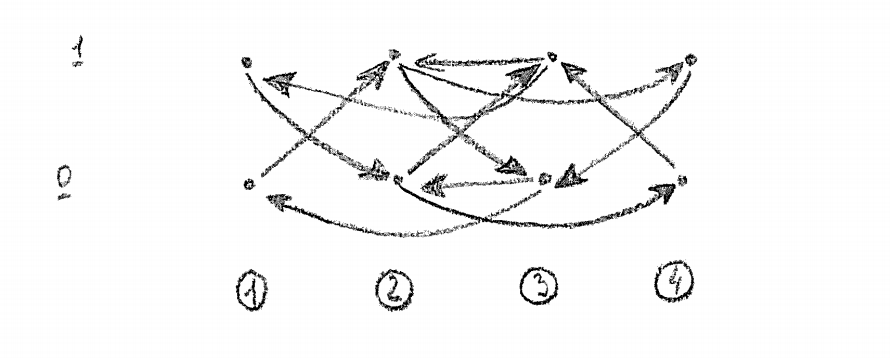
\includegraphics[width=0.9\textwidth]{img/3.png}
		\caption{Вспомогательный граф для примера из раздела 2.2; уровни кратности указаны слева, номера вершин --- снизу.}
		\label{fig:pic_3}
	\end{figure}
	
	Ясно, что во вспомогательном графе уже нет разбиения дуг на множества, все дуги --- обыкновенные, никаких условий на достижимость больше не ставится и все классические алгоритмы могут быть использованы обычным образом. Однако, чтобы удостовериться в последнем, необходимо связать пути на исходном и вспомогательном графах, что и рассматривается в следующей теореме. 
	
	\begin{mydefinition}
		Будем обозначать, что вершина $y$ достижима на некотором графе $G(X,U,f)$, следующим образом: $x \succ G$, при этом будем подразумевать, что она достижима в соответствии с условием на достижимость, если оно задано на графе $G$, и что она достижима в классическом смысле, если на графе $G$ нет условия на нестандартную достижимость.
		В случае недостижимости соответственно будем писать $x \prec G$.
	\end{mydefinition}
	
	\begin{mytheorem}
		Любому пути $\mu'$ на вспомогательном графе $G'$ соответствует путь $\mu$ на графе $G$. При этом вершина $y$ достижима на графе $G$ с учетом условия кратности тогда и только тогда, когда $y^0$ достижима на графе $G'$. 
	\end{mytheorem}
	
	\begin{myproof}
		
		\textit {Необходимость}
		
		Пусть сначала имеем путь $\mu$ длины $n$ на $G$. Доказательство будем проводить индукцией по $n$.
		
		1. \textit {База индукции}
		
		$n = 1$, т.е. путь $\mu$ состоит из одной дуги $u$, $f(u) = (x, y)$. Тогда:
		
		\begin{equation*}
		f'(u) = 
		\begin{cases}
		(x^0, y^0), &\text{$ u \in U_s$, $y^0 \succ G'$, $y \succ G$}\\
		(x^0, y^1), &\text{$ u \in U_o$, $y^0 \prec G'$, $y \prec G$}
		\end{cases}
		\end{equation*} 
		
		Как видим, есть соответствие, база индукции доказана.
		
		2. \textit {Предположение индукции}
		
		Пусть для $ n \leq s$ утверждения верны; докажем их для $ n = s + 1$.
		
		Имеем путь $\mu = \{u_{i_0}, ... , u_{i_s}\}$ такой, что $(p_1 \circ f')(u_{i_0}) = x^0$ и $(p_2 \circ f')(u_{i_s}) \cap \{y^0, ... , y^{p-1}\} \neq \emptyset$. Ясно, что для $\mu / \{u_{i_s}\}$ было выполнено предположение индукции. Обозначим $t = \psi_\mu(s)$.
		
		Сначала предположим, что $u_{i_s} \in U_s$. Тогда при добавлении $u_{i_s}$ в $\mu$ на $G$ кратность не меняется, а в $\mu'$ добавляется дуга $f'(x^t, y^t)$. Т.е. в исходном графе достижимость вершины $y$ совпадает с достижимостью конечной вершины предыдущей дуги, а на вспомогательном графе не произошло перехода на другой уровень кратности, значит, в любом случае достижимость совпадает. 
		
		Теперь рассмотрим случай $u_{i_s} \in U_o$. При добавлении $u_{i_s}$ в $\mu$ кратность увеличилась на единицу, в $\mu'$ при этом добавилась дуга $f'(x^t, y^{(t+1) \mod p})$. Здесь снова два случая:
		
		\begin{itemize}
			\item $t < p - 1$, тогда  $y \prec G$, $y^0 \prec G'$
			\item $t = p - 1$, получаем $\psi_\mu(s+1) = p\mod p = 0$, а на $G'$ стала достижимой $y^0$. Т.о., $y^0 \succ G'$, $y \succ G$.
		\end{itemize}
		
		И снова достижимость для исходного и вспомогательного графов совпадает. 
		
		Значит, предположение индукции верно для всех вариантов, и необходимость доказана.
		
		\textit {Достаточность}
		
		Если $y$ достижима с учётом кратности из $x$, то нa $G$ существует путь $\mu = \{u_0, ... , u_s\}$ такой, что $(p_1 \circ f)(u_0) = x, (p_2 \circ f)(u_s) = y$. Будем строить отображение $\alpha:U\to U'$ по следующим правилам:
		
		\begin{itemize}
			\item каждой дуге $u_i \in \mu$ ставится в соответствие некоторая дуга $\alpha(u_i) \in \mu'$ на $G'$;
			\item $(p_1 \circ f' \circ \alpha)(u_i) = (p_2 \circ f' \circ \alpha)(u_{i-1})$;
			\item дуга $\alpha(u_i)$ задана так, что: 
			\begin{equation*}
			(f' \circ \alpha)(u_0) =
			\begin{cases}
			(x^0, z^0), &\text{$ u_0 \in U_s$}\\
			(x^0, z^1), &\text{$ u_0 \in U_o$}
			\end{cases}
			\end{equation*} 
			
			\item если $f(u_i) = (a, b)$, то $(p_1 \circ f' \circ \alpha)(u_i) \in \{a^0, ... , a^{p-1}\}$ и $(p_2 \circ f' \circ \alpha)(u_i) \in \{b^0, ... , b^{p-1}\}$.
		\end{itemize}
		
		В соответствии с алгоритмом построения вспомогательного графа, отображение $\alpha$ можно построить для любого пути $\mu$; тогда на $G'$ получаем $\mu' = \{\alpha(u_0), ...  \alpha(u_s)\}$. При этом $\mu'$ соединяет $x^0$ и некоторое $y^{t \mod p}$, где $t = \psi_\mu(s)$.
	\end{myproof}
	
	Подчеркнём, что допустимым с учётом кратности путям на $G$ соответствуют только те пути на вспомогательном графе $G'$, которые оканчиваются на нулевом уровне кратности; все прочие вершины соответствуют вершинам на исходном графе в переходном состоянии и не подходят для завершения пути.  
	
	\section{Заключение}
	
	В данном разделе был рассмотрен ход рассуждений, приведший к выделению нового типа условий на графах с нестандартной достижимостью --- глобальных условий. Для них был выделен ряд заметных отличий, что позволяет с уверенностью утверждать, что их нельзя подвести под некоторый частный случай локальных условий. С другой стороны, глобальные условия хорошо вписываются в общую теорию графов с нестандартной достижимостью, для них можно применять аналогичные теоремы и алгоритмы, что, в свою очередь, позволяет рассматривать новые задачи в разрезе уже существующей теории, а не выделять их в некоторую отдельную тему. 
	
	Конкретно задача проверки кратности была выбрана для дальнейшего изучения благодаря простоте поставленного условия на достижимость. Можно предполагать, что наложение в ней дополнительных условий даст получить интересные и изящные результаты, вся совокупность которых будет представлена в следующем пункте данной работы. 
	
	\chapter{Модельная задача с использованием примера глобального условия на достижимость}
	
	\section{Постановка задачи: частный случай}
	
	В данном разделе предлагается рассматривать некоторую модельную задачу, использующую частный случай описанного ранее варианта глобального условия на достижимость, с целью получения более глубоких и практичных выводов. Ее строгая формулировка выглядит следующим образом:
	
	\begin{itemize}
		\item задан орграф $G(X,U,f)$;
		\item $U_* = \emptyset$ и $U^* = U_o = U$;
		\item $\psi_\mu(i) = \sum_{j=0}^i | \mu(j)|\mod p$ задает числовую характеристику пути; 
		\item в начальный момент времени по вершинам $G$ распределены частицы, которые перемещаются по его дугам в каждый момент времени;
		\item переходы частиц на графе определяются матрицей переходов $P$;
		\item на графе задано множество вершин $V_s = \{v_{s_0}, v_{s_1}, ... , v_{s_r}\}$, из которых можно попасть в отдельный от графа сток $s$ с соответствующими вероятностями $\{p_{s_0}, p_{s_1}, ... , p_{s_r}\}$, если путь частицы до вершины из множества является допустимым в соответствии с глобальным ограничением на достижимость: $\psi_\mu(t) = 0$.
	\end{itemize}

	Основной вопрос, который ставится для данной задачи, заключается в том, какое количество частиц покинет граф $G$ в предельном случае. Для начала, попробуем ответить на данный вопрос вне теории графов с нестандартной достижимостью. 
	
	\subsection{Наивный подход}
	
	Для простоты пока будем предполагать, что $G$ является единой компонентой сильной связности. Тогда все вершины графа принадлежат циклам и частицы из любой вершины могут проходить по всем дугам. Сначала приведем нестрогие размышления по задаче, которые далее запишем формально и докажем. 
	
	Для выполнения условия на достижимость для данной частицы нам нужно проложить путь от ее исходной вершины к вершине с возможностью выхода таким образом, чтобы длина этого пути была кратна $p$. Можно добиться этого, например, имея некоторый исходный путь (необязательно допустимый) длины $r$, который мы будем дополнять проходом по какому-нибудь контуру, стартующему из некоторой вершины этого пути. Если мы подберем контур такой, что его длина взаимно проста с $p$, то после ряда проходов по контуру мы сможем получить допустимый путь и для частицы появится возможность выйти из графа. Значит, если мы выясним, при каких условиях возможно подобрать такие контуры, мы сможем ответить на основной вопрос задачи. Эти заключения приводят нас к следующим утверждениям:
	
	\begin{mylemma}
		Пусть $c_1, c_2, ... , c_q $ --- длины простых контуров графа $G$, который является единой компонентой сильной связности, причем $gcd(c_1, c_2, ... , c_q) = 1$. Тогда можно найти такой контур на графе $G$ (возможно, составной), что его длина $c = 1\mod p$.
	\end{mylemma}
	
	\begin{myproof}
		Любой контур можно представить как линейную комбинацию простых контуров: 
		
		\begin{equation*}
		a_1c_1 + a_2c_2 + ... + a_qc_q = gcd(c_1, c_2, ... , c_q) = 1
		\end{equation*}
		
		Данное уравнение разрешимо в целых числах~\autocite{Hasse}, значит, существует набор $a_1, a_2, ... , a_q$ соответствующих целочисленных коэффициентов. В нашем случае коэффициенты должны быть неотрицательны, поскольку они обозначают количество проходов по простому контуру. Но поскольку нам требуется равенство по модулю $p$, все отрицательные коэффициенты можно заменить на положительные, соответствующие по модулю. Таким образом, мы получим линейную комбинацию с неотрицательными коэффициентами, а значит, всегда сможем задать такой контур, что условие на длину будет выполнено. 
	\end{myproof}

	\begin{mytheorem}
		Пусть $c_1, c_2, ... , c_q $ --- длины простых контуров графа $G$, который является единой компонентой сильной связности, и $gcd(p, c_1, c_2, ... , c_q) = 1$. Тогда частицы из всех вершин в предельном случае окажутся в стоке.
	\end{mytheorem}

	\begin{myproof}	
		Для того, чтобы все частицы покинули граф в пределе, необходимо показать, что произвольную вершину всегда можно соединить допустимым путем с вершиной из $V_s$. Как и описано, будем считать, что вершина $v$ соединяется с ней некоторым путем  длины $r$, причем часть этого пути принадлежит некоторому контуру длины $b$. Мы всегда можем считать, что $gcd(p, b) = 1$, т. к. выполняется хотя бы одно из условий:
		
		\begin{itemize}
			\item среди простых контуров графа есть контур длины $c_i$ такой, что $gcd(p, c_i) = 1$ и тогда $b = c_i$, либо
			\item $gcd(c_1, c_2, ... , c_q) = 1$, и тогда в соответствии с доказанной леммой мы можем найти на графе контур $c$ длины  $1\mod p$, значит, $b = c$.
		\end{itemize}
		
		Следовательно, мы можем представить путь частицы в виде $r + bl$, где $l$ – количество дополнительных проходов по контуру. Для того, чтобы этот путь был допустимым, необходимо и достаточно, чтобы выполнялось $r + bl = pm$. Перепишем в виде $r = bl^* + pm$, откуда получим $r = brl^{**} + prm^*$, что представляет собой соотношение Безу~\autocite{Hasse}, домноженное на $r$. Уравнение $1  =bl^{**} + pm^*$ разрешимо в целых числах только при взаимно простых $b, p$. Поскольку это условие выполнено, мы всегда получаем пару целочисленных коэффициентов, удовлетворяющих уравнению. Благодаря неоднозначности их определения мы можем выбрать пару, где коэффициент при $b$ будет отрицательным, а при $p$ – положительным, в соответствии со смыслом данных множителей, и значит, получить допустимый путь до стока из произвольной вершины.
		
	\end{myproof}

	Эти результаты позволяют нам сделать вывод, что при взаимной простоте параметра $p$ и длин простых контуров $G$ все частицы покинут граф в пределе. 
	
	В противном же случае, когда $gcd(c_1, c_2, ... , c_q) = d$, отличному от 1, и $gcd(p,d) > 1$, ясно, что мы cможем получить на графе $G$ только контуры длины, кратной $d$, т.к. 
	
	\begin{equation*}
	a_1c_1 + a_2c_2 + ... + a_qc_q = gcd(c_1, c_2, ... , c_q) = d,
	\end{equation*}	и проход по таким контурам не будет менять кратности пути частиц до вершин из $V_s$. Это значит, что частицы будут однозначно разделены на множества тех, которые покинут граф, и тех, которые будут бесконечно перемещаться по нему, в соответствии с тем, из какой вершины они начали движение в стартовый момент времени. Соответственно, и сами вершины графа можно разделить на множества, но теперь уже отвечающие остатку по модулю $p$ любого пути из данной вершины до вершин из $V_s$. Очевидна и связь между упомянтуыми множествами частиц и множествами вершин: во множество частиц, которые покинут граф, войдут все частицы, начавшие путь из вершин, отвечающих нулю по модулю $p$, а во второе множество войдут все частицы, начальные вершины которых принадлежат оставшимся $p - 1$ множествам. 
	
	Полученные выше результаты позволяют нам теоретически рассчитывать количество частиц, оставшихся в графе $G$ или покинувших его, для любых ориентированных графов, представляющих собой единственную компоненту сильной связности. При этом для проведения такого расчета требуется только набор длин простых контуров исходного графа. Одним из вариантов получения этого набора является обращение к классическому алгоритму~\autocite{Cir}, который позволяет найти множество всех простых контуров за $\mathcal{O}((n + e)(c + 1))$, где $n$ --- количество вершин, $e$ --- количество дуг, $c$ --- количество простых контуров в графе $G$. Дополнительно необходимо только проверить наличие петель в графе, которое данный алгоритм не учитывает, и вычислить длины найденных конутров. 
	
	Таким образом, если 
	
	\begin{equation*}
	a_1c_1 + a_2c_2 + ... + a_qc_q = gcd(c_1, c_2, ... , c_q) = 1,
	\end{equation*}	все частицы покинут граф, а иначе дополнительно нужно будет разметить множества вершин и, следовательно, частиц. Выполнить это можно, например, с помощью BFS.
	
	\subsection{Вычислительный подход}
	
	Приведенное решение имеет слабые стороны: оно достаточно вычислительно сложное, накладывает дополнительные ограничения на задачу и не является универсальным. Попробуем разработать другой метод решения, опирающийся на теорию о нестандартной достижимости на графах. 
	
	В новом подходе к решению сформулированной задачи мы можем использовать результаты, полученные в прошлой главе, т.к. поставленное условие на достижимость является частным случаем разобранного выше глобального условия, когда множество стандартных дуг пусто. Значит, мы можем использовать приведенные ранее алгоритм построения вспомогательного графа и теорему о соответствии путей на исходном и вспомогательном графах.  
	
	Пусть граф $G'$ --- вспомогательный граф для $G$, построенный в соответствии с алгоритмом. Теперь для того, чтобы учесть все условия задачи, нам необходимо выполнить дополнительные манипуляции:
	
	\begin{itemize}
		\item всем дугам $f'(u_i)$ добавим вероятности перехода дуг $u_i$;
		\item множество вершин дополним новой вершиной $s$, являющейся стоком;
		\item вершине $s$ добавим петлю, т.к. все частицы, ушедшие в сток, могут только оставаться в стоке;
		\item обозначим возможность выхода в сток, проведя дуги из каждой вершины множества $\{v^0_{s_0}, v^0_{s_1}, ... , v^0_{s_r}\}$ в $s$;
		\item добавленным дугам сопоставим соответствующие вероятности перехода: $\{p_{s_0}, p_{s_1}, ... , p_{s_r}\}$;
		\item для всех дуг, исходящих из вершин множества $\{v^0_{s_0}, v^0_{s_1}, ... , v^0_{s_r}\}$, кроме входящих в сток, пересчитаем вероятности перехода, 
		домножив их на величины $\{ 1 - p_{s_0}, 1 - p_{s_1}, ... , 1 - p_{s_r}\}$ для каждой такой вершины соответственно, поскольку сумма вероятностей переходов из любой вершины должна быть равна единице.
	\end{itemize}	
	
	Теперь мы получили вспомогательный граф $G'$, полностью описывающий поставленную задачу. Для ее решения, в свою очередь, нам достаточно рассмотреть соответствующую ему матрицу переходов и возвести ее в некоторую достаточно большую степень. Элементы итоговой матрицы будут соответствовать вероятностям перехода частиц между вершинами спустя продолжительное время. Тогда для вершин, у которых вероятность перехода в сток будет близка к единице, мы сможем утверждать, что практически все частицы, расположенные в них в начальный момент времени, покинут граф в пределе. 
	
	Матрицу переходов $P'$ можно сразу получить по графу $G'$. Лучше всего ее записывать, упорядочив вершины вспомогательного графа по уровням кратности, и в конец ставить сток. Тогда, за исключением нижней строки и самого правого столбца, она имеет ярко выраженную блочную структуру: каждый блок отображает вероятности перехода частиц между вершинами двух уровней кратности. Ввиду специфики условия на достижимость, переход осуществляется на один и только на один уровень кратности вверх за такт времени и соответствующий переход по дуге. Поэтому в матрице блоки с ненулевыми элементами есть только на диагонали, расположенной сразу выше главной, и в левом нижнем углу. 
	
	При этом в матрице $P'$ есть два вида блоков, кроме заполненных нулями. В случаях, когда условие на достижимость не выполняется, --- всюду ниже нулевого уровня кратности --- блоки соответствуют уже известной матрице $P$. На нулевом уровне кратности условие выполняется, и там блок соответствует несколько отличающейся матрице, которую мы обозначим как $P^*$. Эта матрица была получена из $P$ путем домножения вероятностей перехода для вершин из $V_s$ на соответствующие кооэффициенты, как описывалось в последнем пункте списка выше.

	Помимо блоков, матрица включает в себя единицу в правом нижнем углу и вектор $S$ на нулевом уровне кратности в самом правом столбце, элементы которого обозначают вероятности выхода из данной вершины в сток.	

	Сначала мы приведём $P'$ в компактном виде, где все элементы до разделительных линий представляют собой блоки размерности $n$, а остальные --- это нулевые вектора длины $n$, вертикальные и горизонтальные, вектор $S$ и единица. Ниже представим более детальную запись матрицы переходов вспомогательного графа $G'$:
	
	\begin{displaymath}
		\mathbf{P'} =
		\left( \begin{array}{ccccc|c}
		0 & P^* & 0 & 0 & ... & S \\
		0 & 0 & P & 0 & ... & \overline {0^T} \\
		0 & 0 & 0 & P & ... & \overline {0^T} \\
		... & ... & ... & ... & ... & ... \\
		P & 0 & 0 & 0 & ... & \overline {0^T} \\
		\hline
		 \overline 0 &  \overline 0 &  \overline 0 &  \overline 0 & ... & 1 \\
		\end{array} \right)
	\end{displaymath}
	
	\begin{table}[H]
		\begin{tabular}{l || c | c | c | c | c}
			& 0,1 0,2 ... 0,n & 1,1 1,2 ... 1,n & ... & p-1,1 p-1,2 ... p-1,n & s \\
			\hline \hline
			0,1 & $\overline 0$ & $P^*_{1,1}$ $P^*_{1,2}$ ... $P^*_{1,n}$ & ... & $\overline 0$ & 0 \\
			... & ... & ... & ... & ... & ... \\
			0,i & $\overline 0$ & $P^*_{i,1}$ $P^*_{i,2}$ ... $P^*_{i,n}$ & ... & $\overline 0$ & $p_{s_i}$ \\
			... & ... & ... & ... & ... & ... \\
			0,n & $\overline 0$ & $P^*_{n,1}$ $P^*_{n,2}$ ... $P^*_{n,n}$ & ... & $\overline 0$ & 0 \\
			\hline \hline
			1,1 & $\overline 0$ & $\overline 0$ & ... & $\overline 0$ & 0 \\
			... & ... & ... & ... & ... & ... \\
			1,i & $\overline 0$ & $\overline 0$ & ... & $\overline 0$ & 0 \\
			... & ... & ... & ... & ... & ... \\
			1,n & $\overline 0$ & $\overline 0$ & ... & $\overline 0$ & 0 \\
			\hline \hline
			... & ... & ... & ... & ... & ... \\
			... & ... & ... & ... & ... & ... \\
			\hline \hline
			p-1,1  & $P_{1,1}$ $P_{1,2}$ ... $P_{1,n}$ & $\overline 0$ & ... & $\overline 0$ & 0 \\
			... & ... & ... & ... & ... & ... \\
			p-1,i & $P_{i,1}$ $P_{i,2}$ ... $P_{i,n}$ & $\overline 0$ & ... & $\overline 0$ & 0 \\
			... & ... & ... & ... & ... & ... \\
			p-1,n & $P_{n,1}$ $P_{n,2}$ ... $P_{n,n}$ & $\overline 0$ & ... & $\overline 0$ & 0 \\
			\hline \hline
			s  & $\overline 0$ & $\overline 0$ & ... & $\overline 0$ & 1 \\
		\end{tabular}
		\caption{Развернутая структура матрицы переходов $P'$}
		\label{tabl:P'}
	\end{table}
	
	Теперь, когда у нас есть матрица $P'$, для которой, как для матрицы переходов вспомогательного графа, условия на достижимость учтены по построению, мы можем возводить ее в достаточно большую степень для анализа ситуации в пределе. Возведение такой матрицы в большую степень можно реализовать разными способами, как достаточно простыми, так и более специфическими, использующими строгую структуру матрицы. К примеру, можно просто последовательно домножать результат на $P'$, можно перемножать результат между собой, удваивая таким образом степень на каждом шаге. Но кроме того, предлагается более специальный способ, принимающий во внимание квазиблочную структуру матрицы $P'$, который может быть полезен в случае больших графа $G$ или параметра $p$.	
	
	Прежде всего, матрицу $P'$ нужно возвести в степень $p$ для приведения в блочно-диагональный вид, за исключением нижней строки и правого столбца. Возведение в степень матрицы диагонального вида сводится к возведению в некоторую степень всех диагональных элементов, а в нашем случае --- блоков на диагонали. Таким образом, для получения практически всех элементов матрицы в степени $rp$ нам достаточно сначала возвести ее в степень $p$ произвольным способом, а потом получить $r$-ые степени матриц размерности $n$, расположенных на диагонали. 
	
	Оcталось рассчитать значения в правом столбце. 
	
	...
	
	После того, как мы возвели матрицу переходов в степень, ответить на вопрос задачи не составляет труда. Все частицы из данной вершины в пределе покинут граф, если в соответствующей строке самого правого столбца матрицы на нулевом уровне кратности получена вероятность, близкая к единице; иначе эти частицы продолжат перемещаться по графу бесконечно. 
	
	\subsection{Теоретический подход}
	
	Однако, когда мы уже построили вспомогательный граф $G'$, получение его матрицы перехода и возведение ее в степень --- не самое оптимальное решение для получения ответа. Поскольку вспомогательный граф по построению учитывает все наложенные условия, никаких внешних ограничений мы для него уже не добавляем. То есть, $G'$ --- обычный граф, и можем использовать для работы с ним классическую теорию графов. 
	
	Найдем в нем компоненты сильной связности: если вершина с нулевого уровня кратности находится в одной компоненте сильной связности со стоком, значит, все частицы из нее покинут граф в пределе. Таким образом получаем то же самое разделение вершин и частиц на множества, которое было описано в первом подходе.  
	
	\newpage % Почему-то библиография накладывалась на таблицу. Быть не должно этого тут.
	
	% Печать списка литературы (библиографии)
	\printbibliography[
	heading=bibintoc%
	,title=Библиография % если хочется это слово
	]
	% Файл со списком литературы: biblio.bib
	% Подробно по оформлению библиографии:
	% см. документацию к пакету biblatex-gost
	% http://ctan.mirrorcatalogs.com/macros/latex/exptl/biblatex-contrib/biblatex-gost/doc/biblatex-gost.pdf
	% и огромное количество примеров там же:
	% http://mirror.macomnet.net/pub/CTAN/macros/latex/contrib/biblatex-contrib/biblatex-gost/doc/biblatex-gost-examples.pdf
	
\end{document}
		
\chaptera{Список литературы}

\begin{itemize}
\bibl{bibl_Romashenko} \textit{А. Ромащенко, А. Румянцев, А. Шень} Заметки по теории кодирования~--- М.: МЦНМО, 2011
\bibl{bibl_Vandervarden} \textit{Б. Л. ван дер Варден} Алгебра~--- М.: Наука, 1979
\bibl{Berzh} \textit{Берж К.} Теория графов и ее применения. — М.: Изд-во иностранной литературы, 1962.
\bibl{bibl_Grosman} \textit{И. Гросман, В. Магнус} Группы и их графы~--- М.: Мир, 1971

\bibl{bibl_Bowditch} \textit{Brian H. Bowditch} A course on geometric group theory~--- М.: World Scientific Publishing Company, 2006
\bibl{bibl_Magnus} \textit{В. Магнус, А. Каррас, Д. Солитэр} Комбинаторная теория групп~---М.: Наука, 1974.
\bibl{bibl_Yandex} \textit{Н.К. Верещагин, Е.В. Щепин} Информация, кодирование и предсказание~---М.: МЦНМО, 2012.
\end{itemize}
\chapter{Приложение}

В приложении мы рассмотрим пример системы, состоящей из случайного процесса с выходом в сток, функционирующим с учётом глобального условия на достижимость. Мы получим состояния этой системы на разных промежутках времени с помощью программной реализации описанного ранее вычислительного подхода и визуализируем результаты. 

Пусть задан ориентированный граф $G$, представленный на рис.\ref{fig:pic_4}:

\begin{figure}
	\centering	
	{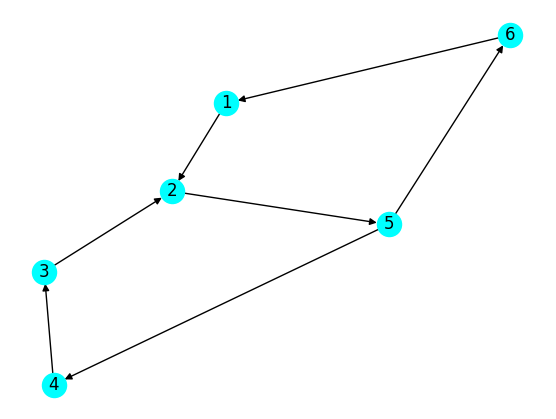
\includegraphics[width=0.9\textwidth]{img/4.png}}
	{Граф $G$}
	\label{fig:pic_4}
\end{figure}

Переходы по всем его дугам равновероятны, и таким образом он задаёт случайный процесс. Положим $k = 2$ и назначим вершину 2 выходной. Его вспомогательный граф $G'$, состоящий из двух изолированных сильно связных компонент (без стока), показан на рис.\ref{fig:pic_5}:

\begin{figure}
	\centering	
	{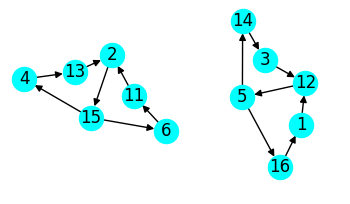
\includegraphics[width=0.9\textwidth]{img/5.png}}
	{Граф $G'$}
	\label{fig:pic_5}
\end{figure}					
\end{document}